\documentclass[10pt,a4paper]{article}
\usepackage[utf8]{inputenc}
\usepackage[spanish]{babel}
\usepackage{listingsutf8}
\usepackage{color}
\usepackage{amsmath}
\usepackage{subfig}
\usepackage{graphicx}
\usepackage{multicol} 
\usepackage{float}
\usepackage{wasysym}
\definecolor{codegreen}{rgb}{0,0.6,0}
\definecolor{codegray}{rgb}{0.5,0.5,0.5}
\definecolor{codepurple}{rgb}{0.58,0,0.82}
\definecolor{backcolour}{rgb}{0.95,0.95,0.92}
\usepackage[top=2cm,bottom=3cm,left=3cm,right=3cm]{geometry}
\setlength{\parskip}{\baselineskip} 

\begin{document}

\setlength{\unitlength}{1cm}
\thispagestyle{empty}
\begin{picture}(18,4)
\put(0,0.2){\includegraphics[scale=.2]{UNAM.jpg}}
\put(11.5,0){\includegraphics[scale=.5]{fc.png}}
\end{picture}
\begin{center}
\textbf{{\LARGE Universidad Nacional Autónoma de México}\\[1cm]
{\LARGE Facultad de Ciencias}}\\[1.8cm]
{\LARGE Práctica 10: Dinámica de fluidos }\\[1.2cm]
\end{center}
\vspace{.7 cm}
\begin{flushleft}{\Large 17 de Octubre 2019  }\\[0.6cm]
\end{flushleft}
\begin{flushright}{\Large{\underline{\textcolor{black}{López Cruz Ángel Jikmé}}}}\\[0.78cm]
\end{flushright}
\begin{flushright}{\Large{\underline{\textcolor{black}{López Velasco Juan Manuel}}}}\\[0.78cm]

\begin{flushright}{\Large{\underline{\textcolor{black}{Robledo Ibarra Emiliano}}}}\\[0.78cm]
\end{flushright}\end{flushright}
\begin{center}
{\Large Profesor: Luis Quintanar Robles }\\[0.4cm]
{\Large Ayudante: Luis Enrique Quintanar Cortés }\\[0.4cm]
\end{center}
RESUMEN: El objetivo principal de la práctica fue describrir las causas de fenómenos relacionados con la dinámica de fluidos utilizando la ecuación de Bernoulli y la ecuación de continuidad. El primer fenómeno fue el vaso invertido de agua el cual se encontró en equilibrio de fuerzas debido a que la presión atmosférica fue más grande a la presión dentro del vaso. El segundo un atomizador en el que el agua se dispersa debido a un cambio de presiones lo que implicó un aumento a la velocidad del líquido. En el tercer experimento, con el Tubo de pitot se midió la velocidad del aire, la cual fue de 1,011 $\pm 0.005 \frac{m}{s}$. El cuarto experimento fue el Tubo de venturi, donde se obtuvo que la velocidad $v_1$ en términos del área de las secciones transversales del tubo en los puntos analizados es $ v_1 = \sqrt{\frac{1.1}{\frac{A^{2}_1}{A^{2}_2}-1}} $. En el quinto, la vela y el vaso de agua tuvo lugar debido a que al estar caliente la vela y taparla el aire se consumió, lo que hizo un cambio de presiones y de altura del líquido. El sexto, el vaporizador al hacer un análisis con la ecuación de Bernoulli se encontró que la presión atmosférica era mayor a la presión dentro del vaporizador. En el séptimo, las pelotas y la corriente de aire fue provocado por un cambio abrupto de presiones, lo que obligó a un cambio de velocidades. El último, cámara de vacío, en el caso de globo fue debido a que la presión fuera del mismo era menor al valor de la presión manómetrica lo que impulsó un cambio de volúmen y en el agua, al cambiar la presión cambió la energía cinética de las partículas del agua.

\normalsize
\newpage


\section{Introducción}

En la Física se estudian diversos cuerpos u objetos los cuales no siempre son rígidos, es por ello que hay ramas de la misma que se dedican al movimiento de distintos cuerpos, una de ellas es la dinámica de fluidos. Los fluidos en movimiento se pueden dividir en dos tipos principales, se conoce como flujo estable o laminar, si cada partícula del fluido sigue una trayectoria uniforme de tal modo que las trayectorias de diferentes partículas nunca se cruzan unas con otras. Dependiendo de la rapidez el flujo del fluido se puede volver turbulento, el cual es irregular y se caracteriza por pequeñas regiones con forma de remolino. [1]

Una de las descripciones utilizadas para los fluidos en movimiento es la ecuación de continuidad para los fluidos, la cual afirma que el producto del área y la rapidez del fluido en todos los puntos a lo largo de una tubería es constante para un fluido incompresible, dicho de otra forma: 

\begin{equation}
	A_1 v_1 = A_2 v_2 = cte
\end{equation}

Donde para cualesquiera dos puntos del fluido en movimiento se cumple;  es equivalente afirmar que el volumen de fluido que entra por un extremo en un intervalo de tiempo dado es igual al volumen que conduce al otro extremo del tubo (si no hay fugas).

Existe otra relación muy importante entre los fluidos que es la ecuación de Bernoulli y se aplica a fluidos ideales (estacionario, irrotacional, no viscoso e incompresibles) y se enuncia de la siguiente manera:

\begin{equation}
	P + \frac{1}{2}\rho v^2 + \rho g y = cte 
\end{equation}

Y de ella se puede ver que, en dado caso de que se cumpla, la presión de un fluido disminuye conforme la rapidez del mismo aumenta y además, la presión disminuye conforme aumenta la elevación.[1] De esta forma, con estas dos ecuaciones es posible modelar una gran cantidad de fenómenos que ocurren en fluidos en movimiento a velocidades bajas. Para este reporte se probaron dos fluidos: aire y agua. Ambos a velocidades moderadas de tal forma que bajo condiciones no extraordinarias podría aplicarse hipótesis como: estacionario o irrotacional e incluso  incompresibles. 

\newpage
\section{Procedimiento}
Como se realizaron ocho experimentos se describirán los mismos por separado.

\subsection*{El vaso que no se derrama.}
Para este experimento se tomó un vaso de vidrio sin distinción alguna, posteriormente se llenó a la mitad de su capacidad con agua del grifo, una vez hecho esto se le cubrió con una cubierta de plástico y, uniendo ambos con fuerza se volteó este conjunto y después de estar seguros de que estuviera en equilibrio se sostuvo del vaso apartando la mano de la placa de plástico.
\begin{figure}[H]
\includegraphics[scale=0.22]{vaso1.png}
\centering
\caption{1. Vaso con agua 2.Tapa plástica.}
\end{figure}

\subsection*{Atomizador.}
Para el atomizador se decidió no desperdiciar más agua y del sistema anterior se le retiró la tapa una vez volteado, se tomó el esqueleto del atomizador que consistía en dos tubos, uno conectado al agua y el otro que recibiría aire a través de una bomba de aire. Se probaron tres formaciones distintas hasta que la tercera funcionó: la primera a mitad del tubo conector al líquido, la segunda formando un ángulo recto entre ambas boquillas y la tercera completamente en contacto con el tubo conectado al agua pero la mitad de él lo sobrepasaba.
\begin{figure}[H]
\includegraphics[scale=0.22]{atomizador1.png}
\centering
\caption{1. Vaso con agua 2. Esqueleto del atomizador. 3. Bomba de aire.}
\end{figure}

\subsection*{Tubo de Pitot}
En este experimento se utilizó un tubo de Pitot para medir la velocidad con la que una compresora expulsa aire. 
Para ello se conectó el tubo de Pitot a un manómetro de dos ramas abiertas y con una compresora se hizo circular aire a través del tubo. 
Se midió una diferencia de alturas (medida directa) entre las columnas del fluido (agua) contenido en las ramas del manómetro.
\begin{figure}[H]
\includegraphics[scale=0.05]{4.jpg}
\centering
\caption{Diferencia de alturas entre las columnas de fluido del manómetro.}
\end{figure}

\subsection*{Tubo de Venturi}
En este experimento se utilizó un tubo de Venturi para medir la velocidad con la que el agua sale del grifo (en las instalaciones del Laboratorio de Calor, Ondas y Fluidos II, Facultad de Ciencias, UNAM).
Se conectó el tubo de Venturi a un manómetro de dos ramas abiertas , además, con una manguera de plástico, se conectó el tubo al grifo. Se hizo fluir agua a través del tubo y se midió (medida directa) una diferencia de alturas entre las columnas de fluido (agua) contenidas en las ramas del manómetro. 
\begin{figure}[H]
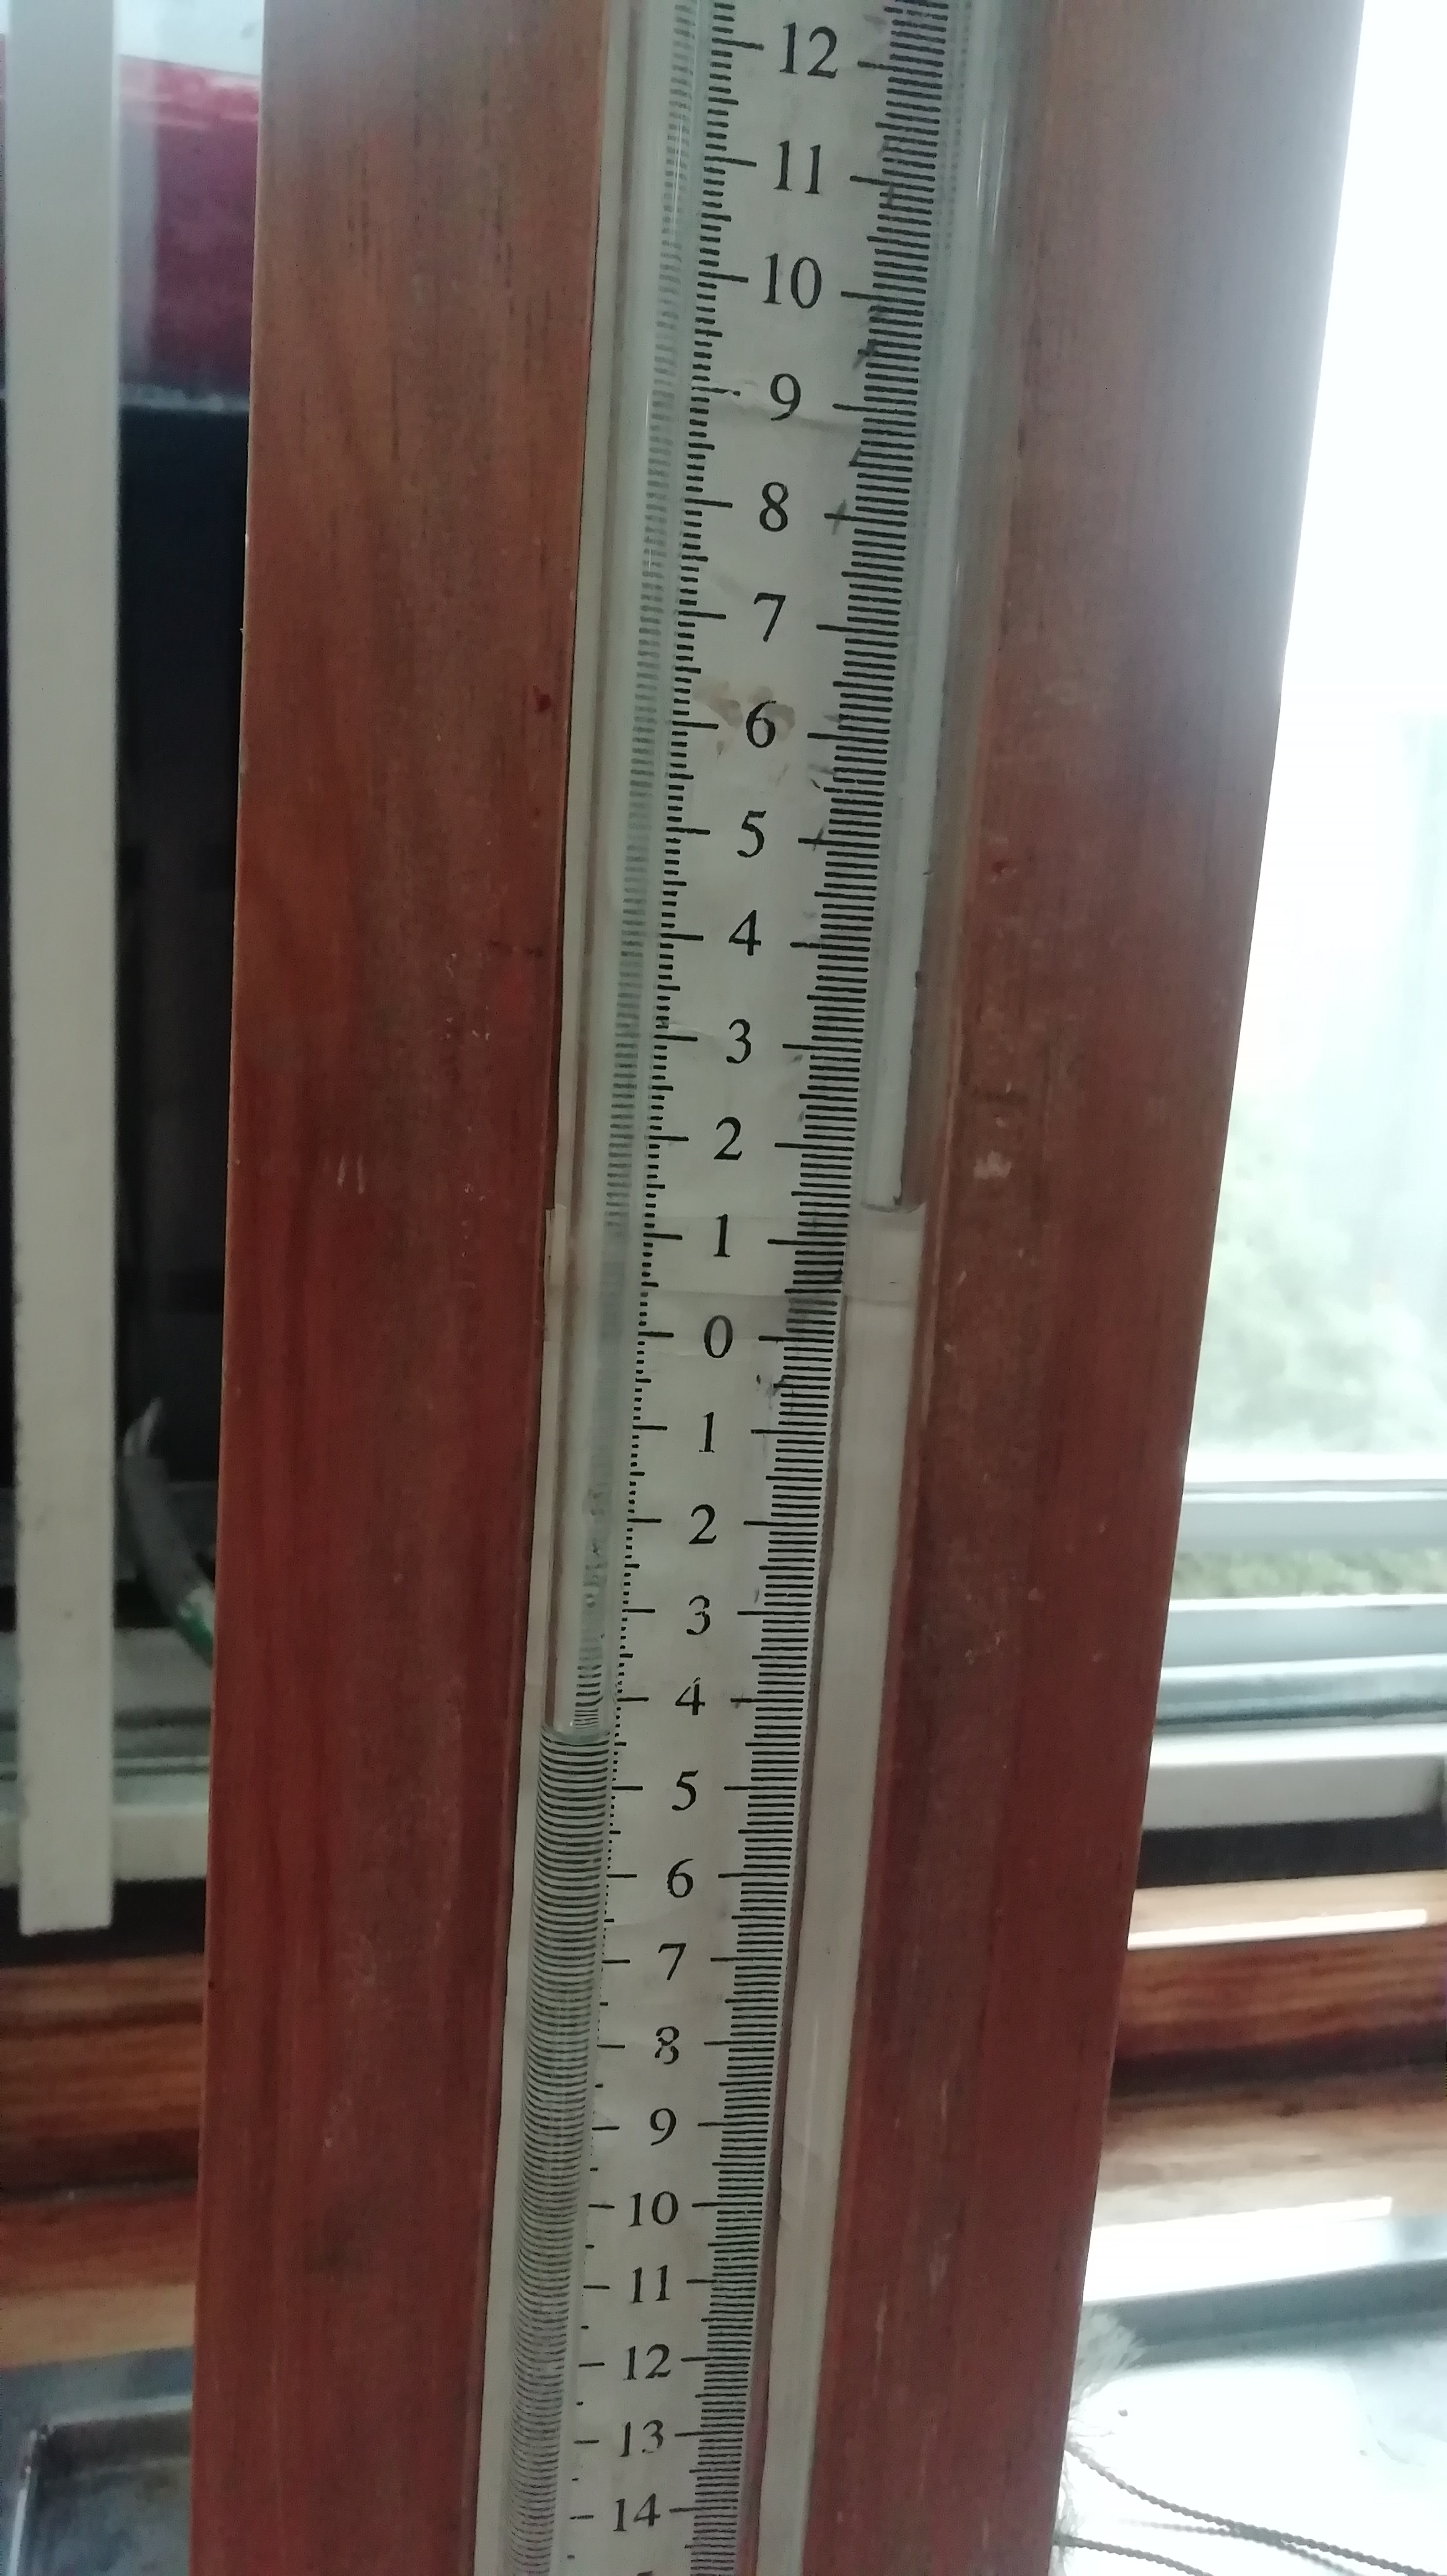
\includegraphics[scale=0.05]{5.jpg}
\centering
\caption{Diferencia de alturas entre las columnas de fluido del manómetro.}
\end{figure}


\subsection*{Caja de Petrit y vela}
Con plastilina se colocó una vela en una caja de Petrit aproximadamente en el centro de la base. Luego se vertió agua en la caja hasta que esta estuviese llena aproximadamente hasta la mitad de su capacidad.

Se encendió la vela con un cerillo y posteriormente se tomó el vaso de vidrio utilizado en experimentos anteriores y se colocó en la caja, de modo que la vela quedó contenida en el interior del vaso.

\begin{figure}[H]
\includegraphics[scale=0.04]{vela.jpg}
\centering
\caption{1. Caja de Petrit. 2. Vela. 3. Vaso de vidrio.}
\end{figure}

\subsection*{Vaporizador}
Se llenó menos de la mitad un vaporizador con agua y conectado a su manguera respectiva, en una parrilla eléctrica se dejó hervir por unos 10 minutos (procurando que el agua no se acabara). En un vaso de vidrio se colocó agua a temperatura ambiente, al término de los 10 minutos, se sacó de la parrilla el vaporizador e inmediatamente se metió la manguera del vaporizador dentro del agua del vaso, enseguida se observó lo que sucedió.

\begin{figure}[H]
\includegraphics[scale=0.15]{1.jpeg}
\centering
\caption{1. Vaso de agua 2. Manguera de plástico 3.Vaporizador 4. Parrilla eléctrica}
\end{figure}

\subsection*{Pelotas que se unen.}
En este experimento se utilizó un sistema ya construido que consistió en dos pelotas de ping pong (semejantes) que por medio de un hilo se colgaron del techo a una altura similar; una vez sujetas se hizo pasar aire a una gran velocidad gracias a una compresora con una boquilla especial que lo redirigiese. Se hizo pasar el aire inyectado dirigiéndolo gracias a la boquilla.
\begin{figure}[H]
\includegraphics[scale=0.3]{pelotas.png}
\centering
\caption{1. Pelotas suspendidas 2. Boquilla que redirige de la compresora.}
\end{figure}

\subsection*{Cámara de vacío} 
En una cámara de vacío se colocó un globo (con poco aire), un vaso de vidrio lleno de agua. Se cerró y, con una bomba de vacío se extrajo el aire que contenía, se observó y discutió lo que pasó con el globo y el agua. 
\begin{figure}[H]
\includegraphics[scale=0.18]{2.jpeg}
\centering
\caption{1. Globo 2. Vaso con agua 3. Cámara de vacío 4. Compresor de aire}
\end{figure}


\section{Resultados.}
Para la sección de resultados se muestran los fenómenos obtenidos mediante fotos que captaron el fenómeno a observar.

\begin{figure}[H]
    \centering
    \subfloat[Antes de hervir.]{{\includegraphics[width=5cm]{1)v.jpeg} }}%
    \qquad
    \subfloat[Después de hervir.]{{\includegraphics[width=5cm]{2)v.jpeg} }}%
    \caption{Efecto observado en el vaporizador, en la figura a) se ve antes de hervir y en la b) después de hervir.}%
    \label{fig:example}%
\end{figure}

\begin{figure}[H]
    \centering
    \subfloat[Antes]{{\includegraphics[width=5cm]{1)p.png} }}%
    \qquad
    \subfloat[Durante]{{\includegraphics[width=5cm]{2)p.png} }}%
    \caption{Fenómeno registrado en el experimento de las pelotas colgadas, antes y durante el momento de echar aire.}%
    \label{fig:example}%
\end{figure}

\begin{figure}[H]
\includegraphics[scale=0.2]{Efectovela.jpeg}
\centering
\caption{Efecto después de haber colocado el vaso de tal forma que cubriese la vela.}
\end{figure}













\begin{figure}[H]%
    \centering
    \subfloat[Antes de retirar aire.]{{\includegraphics[width=5cm]{1)8.jpeg} }}%
    \qquad
    \subfloat[Después de retirar aire.]{{\includegraphics[width=5cm]{2)8.jpeg} }}%
    \caption{Efecto observado en el octavo experimento, antes y después de retirar el aire.}%
    \label{fig:example}%
\end{figure}

\newpage
\section{Análisis de resultados.}
\subsection*{Primer experimento}
Se observó que al invertir el vaso que contenía agua no se derramaba y de hecho el sistema era estable de forma que era posible sujetar sólo el vaso sin preocuparse por qué la lámina plástica se cayera. 

\begin{figure}[H]
\includegraphics[scale=0.3]{vvaso.jpg}
\centering
\caption{Diagrama del vaso.}
\end{figure}


Para explicar este fenómeno se propone revisar la hidrostática, debido a que el experimento se encuentra en un espacio abierto, se considera la presión atmosférica. Una vez teniendo el agua dentro del vaso se le colocó una tapa para poder ''aislar'' dicho líquido de manera que ya no afectase dentro la presión atmosférica y solamente hubiera aire y agua dentro del vaso; ya tapado se invirtió y es aquí donde aplicamos la ecuación hidrostática usando $v=0$ y la altura de referencia para la tapa $h_1=0$: $P_{atm} = P_0 + \rho g h_2$. Donde la presión dentro ($P_0$) la ocasiona el aire contenido y el segundo término se debe al fluido contenido. De esta forma tenemos dos fuerzas por unidad de área sobre el mismo eje (vertical) y como la presión atmosférica es mayor que aquella dentro del vaso, estas se encuentran en equilibrio y la tapa no se cae.




\subsection*{Segundo experimento}
En el segundo experimento se probaron tres formaciones distintas hasta que la tercera funcionó: la primera a mitad del tubo conector al líquido, la segunda formando un ángulo recto entre ambas boquillas y la tercera completamente en contacto con el tubo conectado al agua pero la mitad de él lo sobrepasaba. Y sólo funcionó la tercera.

La razón por la cual el tercer experimento funcionó se explica, gracias a dos ecuaciones, de la siguiente manera: la primera parte se debe a que $Av = cte$ ya que al hacer pasar aire por un tubo que reduce su área transversal éste aumenta su velocidad (acelera) y este aumento de velocidad es importante para que en la ecuación $P + \frac{1}{2}\rho v^2 + \rho g h = cte$, donde se analizan dos puntos: dentro del agua (cerca del extremo del tubo) y fuera de ella (en el otro extremo del mismo tubo). Sabemos que ambos puntos tienen a la presión atmosférica aplicada de ambas partes por lo que es innecesario contarla pero en uno la velocidad es mucho mayor lo cual reduce la presión y al reducir la presión de dicho punto el líquido tiende a subir de forma que la ecuación antes escrita se cumpla y por último el líquido que entra en contacto con el aire se disperse por el mismo; es de hecho como los popotes funcionan (por un cambio en la presión en un punto). El porqué de la configuración es gracias a que es necesario cambiar la presión en un punto directamente en contacto con el agua.

\subsection*{Tercer experimento. Tubo de Pitot}
Se observó que al hacer fluir aire a través del tubo se produjo una diferencia de alturas entre las columnas de líquido en las ramas del manómetro, lo que indica una diferencia de presiones en dos puntos distintos del tubo. Del siguiente esquema se tiene que 
\begin{figure}[H]
\includegraphics[scale=0.09]{pitot.jpg}
\centering
\caption{Tubo de Pitot}
\end{figure}
considerando la ecuación de Bernoulli, se tiene una presión $P_b$ en el punto $b$ y, además, la velocidad $v_b$ en dicho punto es cero pues, al fluir el aire por el tubo desplaza la columna de líquido del manómetro hasta estar en equilibrio. Para el punto a se tiene una presión $P_a$ y, en este punto el aire fluye con una velocidad $v_a$ distinta de cero, que es la velocidad que se desea obtener.  
Debido a que la diferencia altura entre el punto $a$ y el punto $b$ es muy pequeña se despreciará el término $\rho g h$ en ambos lados de la ecuación. 
Así, despejando $v_a$ de la ecuación de Bernoulli se tiene que $$v_a =\sqrt{\frac{2(P_b - P_a)}{\rho_a}}$$ donde la diferencia de presiones $P_b - P_a$ es igual a la presión hidrostática debido a la diferencia de altura $h$ en las columnas de líquido del manómetro, es decir $P_b - P_a = \rho_f g h$.

Considerando la densidad del aire $\rho_a$ como 0.92 $kg/m^3$, la densidad del agua $\rho_f$ como 1 $kg/m^3$ y la diferencia de altura (medición directa) $h$ como 0.048 $\pm$ 0.0005 m se calculó la velocidad del aire.

La velocidad del aire medida fue de $v_a = 1.011 \pm 0.005 m/s$ (la incertidumbre asociada se calculó utilizando el método de propagación de incertidumbre para funciones de una variable).

\subsection*{Cuarto experimento. Tubo de Venturi}
\begin{figure}[H]
\includegraphics[scale=1.4]{venturi.png}
\centering
\caption{Tubo de Venturi}
\end{figure}


Se observó que al hacer fluir agua del grifo a través del tubo de Venturi se producía una diferencia de alturas entre las columnas de fluido en las ramas del manómetro.
Utilizando la ecuación de Bernoulli, como la diferencia de alturas entre los dos puntos a analizar en el tubo es muy pequeña, simplificamos el término $\rho g h$ de ambos lados de la ecuación, así $$ P_1 + \frac{1}{2} \rho v^{2}_1 = P_2 + \frac{1}{2} \rho v^{2}_2 $$ 

Expresando la diferencia en términos de la diferencia de alturas en las ramas del manómetro se tiene que $\Delta P=\rho_a g h$. La diferencia de altura fue medida (medición directa) obteniendo un valor de $h=0.059 m$ y, considerando $\rho_a = 1 kg/m^3$ y $g=9.8m/s^2$ se tiene que $\Delta P = 0.578 \pm 0.05 Pa$.

Así $$\Delta P = \frac{1}{2}\rho (v^{2}_2 -v^2_1) $$
Sustituyendo el valor de $\Delta P$ y despejando la diferencias de velocidades al cuadrado de la ecuación se tiene que $$ v^{2}_2 -v^2_1 = 1.1 \pm 0.1 m^2/s^2 $$

Utilizando la ecuación de continuidad se pueden relacionar la velocidad $v_1$ con la velocidad $v_2$, donde $$ v_2 = \frac{A_1 v_1}{A_2}$$
Finalmente, se tiene que la velocidad $v_1$ en términos del área de las secciones transversales del tubo en los puntos analizados es $$ v_1 = \sqrt{\frac{1.1}{\frac{A^{2}_1}{A^{2}_2}-1}} $$

\subsection*{Quinto experimento.}
Se observó que el nivel del agua dentro del vaso subía a la vez que la vela se apagaba. 
Después de un tiempo determinado la vela se apagó y el nivel del agua dentro del vaso se estabilizó, es decir, el sistema estuvo en equilibrio.
\begin{figure}[H]
\includegraphics[scale=1.2]{vaso2.JPG}
\centering
\end{figure}


Para el análisis de qué sucede en este experimento se utilizó la ecuación de Bernoulli.
Al inicio, el sistema formado por la caja de Petrit, el agua contenida en ella y la vela encendida se encuentra sometido a la presión en el laboratorio $P_L$. Posteriormente se modificó el sistema agregando el vaso de vidrio. 
Este cambio en el sistema produjo una diferencia de presiones entre el fluido (agua) que se encontraba fuera del vaso sometido a la presión del laboratorio y el fluido dentro del vaso, sometido a la presión dentro del vaso $P_v$. 
Se observó que el fluido dentro del vaso aumentó su altura con respecto a la altura inicial (se considerará a la altura inicial como cero), lo que indica que la presión dentro del vaso $P_v$ era menor a la presión del laboratorio $P_L$.
Después de un tiempo dado el sistema se equilibra, de modo que se puede despreciar el término $\rho g h$ de la ecuación de Bernoulli.
Así, se tiene que $P + \frac{1}{2} \rho v^2 = cte$ y, de este modo se puede hallar la altura h que alcanzará el fluido dentro del vaso debido a la diferencia de presiones suponiendo que en un punto $a$ el cual ubicaremos en la boca del vaso en contacto con la caja de Petrit la altura es cero y sólo interviene la presión $P_L$ y que en el punto $b$, el cual estará a la altura $h$ a la que llegue el fluido, la presión a la que está sometido es $P_v$. Expresando lo anterior en términos de la ecuación de Bernoulli se tiene $$ P_L - P_v = \rho g h $$
Reordenando la ecuación anterior se obtiene la altura $h$ que alcanza el fluido dentro del vaso $$ h= \frac{\Delta P}{\rho g} $$


\subsection*{Sexto experimento}
El agua del vaso de vidrio fue succionada por el vaporizador.
Por el principio de Bernoulli se describió que sucedió.
\begin{figure}[H]
\includegraphics[scale=0.65]{Vaporizacion.png}
\centering
\end{figure}
En el vaso de vidrio, se denotó como la posición ''a'', y como posición ''b'' a la entrada del vaporizador con el tubo de plástico.

$Po_{a}+\frac{\rho*(V_a)^2}{2}+\rho*g*A$ = $Po_{b}+\frac{\rho*(V_b)^2}{2}+\rho*g*(A+B)$

Podemos eliminar $\rho*g*A $. Despejemos la velocidad en B.

$Po_{a}-Po_{b}+\frac{\rho*(V_a)^2}{2}-\rho*g*B$ = $\frac{\rho*(V_b)^2}{2}$

$V_b$ = $\sqrt{2(\frac{Po_a-Po_b}{\rho})+(V_a)^2 -2*g*B}$

Por la ecuación de continuidad tenemos que $A_a*V_a=A_b*V_b$ como el $A_a>>A_b$ entonces $V_a<<V_b$ podemos despreciar el valor de la $(V_a)^2$

$V_b$ = $\sqrt{2(\frac{Po_a-Po_b}{\rho})-2*g*B}$

Como la velocidad en b es positiva, entonces tenemos que:
$2(\frac{Po_a-Po_b}{\rho})-2*g*B >0$

Despejemos $Po_a$

$Po_a>Po_b+g*B*\rho$

Como $Po_b+g*B*\rho$ son dos valores positivos entonces $Po_a>Po_b+g*B*\rho>Po_b$ 

Como la presión en a es la presión atmosférica, entonces decimos que la presión atmosférica es mayor que la presión en b dentro del vaporizador.


En un inicio en el vaporizador la presión dentro era la presión atmosférica y no existía vapor, cuando llegó al punto de ebullición el vapor del agua con la presión atmosférica se igualó, pero las partículas de vapor al recibir mayor calor, aumentó su temperatura y recordemos que la temperatura es la energía interna de un sistema termodinámico, es decir las partículas aumentaron su velocidad, pero además recordemos que estaba hirviendo, al dejar de recibir calor, se enfrió su interior y la  presión bajó, se tomó al punto B y por la ecuación de Bernoulli, $Po_b+ \frac{\rho V_o}{2}+ \rho* g*(A+B)=Pf_b+ \frac{\rho V_f}{2}+ \rho* g*(A+B)$ se eliminó el término de la altura y se obtuvo $Po_b+ \frac{\rho V_o}{2}=Pf_b+ \frac{\rho*V_f}{2}$ Como aumentó la velocidad de las partículas de vapor de agua para que se cumpliera dicha relación la presión tuvo que disminuir, por lo tanto llegamos a la conclusión que la presión en b disminuyó y como la presión en un principio era la atmosférica, entonces la presión final era menor a la atmosférica, lo cual coincide con lo dicho en el análisis de datos, por lo tanto debido a esa diferencia de presiones, el agua del vaso de vidrio ingresó al vaporizador.

\subsection*{Séptimo experimento (dos pelotas que se juntan).}

Para este experimento se probaron dos configuraciones distintas ambas con el mismo resultado, apenas se hizo pasar aire entre ambas pelotas se juntaron y luego se retiró el aire de ese punto para que ambas volviesen a su estado original. 

En primer lugar es notorio que las velocidades en dos puntos: entre ambas pelotas y en su lateral son ambas distintas. Y la velocidad entre ellas debido a que se hizo pasar aire modificó este estado de equilibrio. Ambas se encontraban a la misma altura por lo que el punto de referencia hace que el término $\rho g y $ sea idéntico en ambos puntos a analizar. La razón $P_1 + \frac{1}{2} \rho v_1^2 = P_2 + \frac{1}{2} \rho v_2^2$ nos dice que debido a que la velocidad del fluido entre ambas pelotas es mucho mayor que fuera de este punto. Es por ello que para que la ecuación tenga sentido, la presión en dicho punto es menor en comparación del exterior.

En este caso se puede ver como en el experimento dos (atomizador) que hay una corriente de aire a grandes velocidades que en analogía a dicho experimento aquí también el aumento o cambio de velocidad se relaciona con un cambio en la presión de forma que la presión en la línea que una a ambas pelotas se divide en dos: la presión atmosférica que sufren los objetos al estar expuestos al aire y la presión menor en medio de ambas que se debe al aire inyectado y su velocidad. Este cambio tan súbito de presiones hace que, como cada pelota se encuentra bajo el efecto de la presión atmosférica, se muevan hacia la otra debido a que entre ellas hay una presión menor. No debemos olvidar que este efecto está íntimamente relacionado con el hecho de que  un a presión es una fuerza por unidad de área que dentro de un fluido es experimentada en todas direcciones.

\subsection*{Octavo experimento: Cámara de vacío}

Se notó que al substraer el aire de la cámara de vacío, el globo empezó a aumentar de volúmen y el agua empezó a hervir.
Es decir, la presión del globo en su exterior disminuía, entonces la presión en su interior lograba aumentar el volúmen, en el caso del agua por la ecuación de Bernoulli tenemos que $Po+ \frac{\rho V_o}{2}+ \rho* g*(h)=Pf+ \frac{\rho V_f}{2}+ \rho* g*(h)$  pero como el agua no cambio de lugar podemos eliminar el término $\rho* g*(h)$ entonces obtenemos que $Po+ \frac{\rho V_o}{2}=Pf+ \frac{\rho V_f}{2}$ y como la presión al final disminuye, entonces debe aumentar la velocidad, pero como el agua no está en movimiento, entonces debe cambiar la energía cinética de las partículas, es decir, aumenta su energía cinética y empieza a hervir.

El punto de ebullición de un líquido es la temperatura a la cual la presión de vapor del líquido iguala a la presión atmosférica, en la cámara de vacío se disminuyó la presión dentro de la cámara lo que provocó que el agua alcanzara la ebullición, en el caso del globo, como la presión manométrica (en el interior del globo) fue mayor a la presión exterior, lo que provocó que el globo cambiara de tamaño.








\section{Conclusiones.}
En los ocho experimentos fue posible observar diversos fenómenos que involucraron directamente el comportamiento de un fluido bajo ciertos estados, estos efectos estaban íntimamente relacionados a cada fluido puesto que no se comportaron de manera idéntica aunque sí algo similar. Observamos que aprovechando las condiciones iniciales y realizándoles ciertos cambios en aspectos como el área transversal por la que fluye influyen en otro aspectos. Como se explica en la introducción, es posible asociar a estos experimentos con la rama de la física que estudia los fluidos en movimiento puesto que tanto el aire como el agua son ambos fluidos. A pesar de haber obtenido descripciones cualitativas de lo ocurrido, es posible describir los fenómenos ocurridos bajo las hipótesis adecuadas. 

En experimentos como el atomizador, las pelotas, el tubo de Pitot y el tubo de Venturi se observó que la velocidad de un fluido puede generar cambios en la presión y, además de ello, esta velocidad no sólo depende de las condiciones iniciales sino que puede variar dependiendo del recipiente en el cual es confinado el fluido o dónde se le hace transitar. La velocidad es constante sobre un área igual independiente de la figura, sin embargo, conforme se le hace transitar en áreas menores tiende a aumentar la velocidad; cabe resaltar que el agua y el aire son dos fluidos distintos puesto que por una parte se considera incompresible al agua, el aire si lo es y por tanto tienen distintos rangos de valores para las velocidades en los cuales se cumple. 

Además, con las ecuaciones utilizadas bajo las suposiciones hechas en la introducción sobre las características de los fluidos, no sólo se pueden describir y explicar diversos fenómenos físicos sino que, también se puede predecir el efecto que se tendrá al variar una (o varias) de las condiciones iniciales del sistema en cuestión.


\begin{thebibliography}{x}

\bibitem{Baz} \textsc{Serway, A. }(1997). \textit { En physics for scientist engineers}. Orlando Florida.

\bibitem{Baz} \textsc{Resnick, R }(2001). 
\textit{ Dinámica de fluidos . En Física 1}. México.


\end{thebibliography}
\end{document}
